\chapter{Descripción del algoritmo}
\par En este capítulo se describe el algoritmo desarrollado para la resolución de ecuaciones que definen el proceso de transferencia de calor en cada sección del horno, haciendo referencia los métodos numéricos utilizados y descritos en los anexos. También se describen las características físicas del horno a simular.

\section{Algoritmo}
\par El diagrama mostrado en la Figura \ref{fig:diagrama-algo}, representa la secuencia del algoritmo. Consta de un ciclo externo que incluye una sección de combustión, sección de radiación, sección de escudo y sección de convección. Su descripción será desarrollada en las subsecciones consiguientes.
\begin{figure}[hbt]
\begin{center}
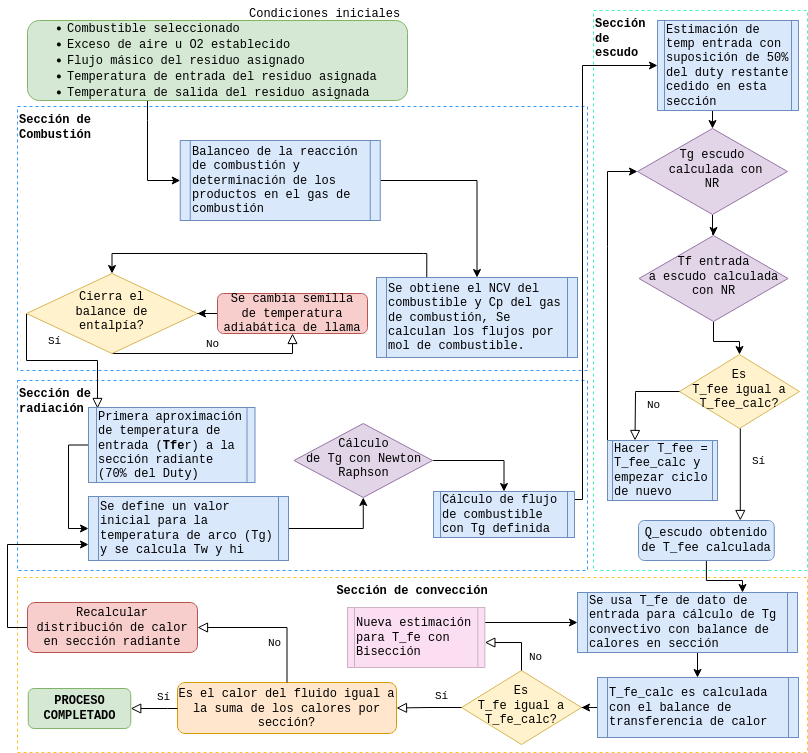
\includegraphics[scale=0.45]{images/diagrama-algo}
\caption[Diagrama de algoritmo]{Diagrama descriptivo del algoritmo desarrollado para el simulador.}
\label{fig:diagrama-algo}
\end{center}
\end{figure}

\par Datos iniciales no editables en el simulador:
\begin{itemize}
    \item Dimensiones del horno y configuración de los tubos en la cámara de combustión.
    \item Propiedades físicas y dimensiones de los tubos y aletas.
\end{itemize}
\par Datos de entrada modificables en la interfaz de usuario:
\begin{itemize}
    \item Flujo másico del fluido de proceso y sus propiedades a la entrada y salida del horno: temperatura, gravedad específica, calor específico, conductividad térmica y viscosidad.
    \item Composición del combustible y su temperatura de entrada.
    \item Exceso de aire, humedad relativa y temperatura del aire ambiental.
\end{itemize}
\par Las propiedades del fluido a temperaturas intermedias son calculadas mediante una interpolación lineal, excepto para la viscosidad, en la que se usa la siguiente interpolación exponencial:
\begin{equation}
\begin{gathered}
    \mu(t) = A * e^{B/t} \\
    B = \frac{ln(\mu_1/\mu_2)}{1/t_1 - 1/t_2} \\
    A = \mu_1 * e^{-B/t_1};
\end{gathered}
\end{equation}
\par Donde:\\
$t_1$ y $t_2$ son la temperatura del fluido a la entrada y salida del horno respectivamente.\\
Y $\mu_1$ y $\mu_2$ son la viscosidad del fluido a la entrada y salida del horno respectivamente.
\subsection{Sección de combustión}
\par En esta sección del algoritmo se realizan los cálculos de la composición del gas de combustión, sus propiedades físico-químicas y el poder calorífico del combustible; a través del balance de masa y energía a partir los componentes del combustible y considerando combustión completa.
\par Las propiedades físico-químicas calculadas son, la capacidad calorífica específica, peso molecular, viscosidad y conductividad térmica.
\par En el simulador se programaron funciones cuadráticas con dependencia en la temperatura para obtener la viscosidad y conductividad de los componentes del gas de combustión, los coeficientes para cada una de las propiedades se obtuvieron con los datos del Instituto Nacional de Estándares y Tecnología (NIST)\cite{nist}, y son alojados en una base de datos interna del simulador, el código desarrollado para las ecuaciones se muestra en los apéndices.
\par Al ser sistemas multicomponentes, las propiedades son la suma de las propiedades individuales por sus fracciones molares correspondientes.
\begin{gather}
    Propiedad_{sustancia} = \Sigma Propiedad_{i} * x_i \\
    k = c_{k0} + c_{k1}*T + c_{k2}*T^2 \\
    \mu = c_{\mu0} + c_{\mu1}*T + c_{\mu2}*T^2
\end{gather}
\par Donde:\\
$c_{k0,k1,k2}$ y $c_{\mu0,\mu1,\mu2}$ son las constantes de conductividad y viscosidad para cada componente respectivamente.
\par En caso de la capacidad calorífica (ec. \ref{eq:cp}) se usa la ecuación cúbica mostrada en el libro de Borgnakke y Sonntag \cite{bib:vanwylen}, para cada componente: 
\begin{equation}
\label{eq:cp}
    Cp = cp_0 + cp_1*\theta + cp_2*\theta^2 + cp_3*\theta^3
\end{equation}
\par Donde:\\
$\theta$ = Temperatura [K]/1000
\par Finalmente se calcula la relación aire/combustible con la ecuación \ref{eq:ac}, la temperatura adiabática de llama y el poder calorífico neto del combustible (NCV) de la ecuación \ref{eq:cv}.

\subsection{Cálculo térmico del horno}
\par En esta sección del algoritmo se inicia el ciclo encargado de resolver el balance global de energía del horno, calculando el calor transferido en cada sección del horno, es donde se define la distribución de calor de la zona radiante y se varia este valor para alcanzar la tolerancia deseada con un método iterativo aplicado a la siguiente ecuación.
\begin{equation}
\label{eq:ciclo_externo}
\frac{(Q_{absorbido} - Q_{calc})}{Q_{calc}} \approx 0
\end{equation}
\par Donde:\\
$Q_{absorbido} = m_{f} * Cp_{f} * (T_{f_s}-T_{f_e})$ \\
$Q_{calc} = Q_{RAD} + Q_{ESC} + Q_{CONV}$; calculado por los modelos de transferencia de calor descritos.
\par Lo que se traduce en que el calor absorbido por el residuo debe ser igual al calor calculado en cada una de las secciones del horno.
\par En las siguientes subsecciones se detalla el algoritmo para cada zona del horno.

\subsection{Sección de radiación}
\par En esta zona se deben determinar tres variable desconocidas: El calor cedido al fluido $Q_{RAD}$, la temperatura de entrada del fluido a esta zona $T_{fer}$ y la temperatura efectiva de los gases de combustión $T_g$.

\par \textbf{Suposición A}: El valor de la temperatura de entrada del fluido a esta sección resulta de suponer inicialmente una absorción del calor del horno en la zona radiante igual al 70\%$Q_{absorbido}$; el resto es distribuido entre la zona escudo y zona convectiva, en consecuencia (ec. \ref{eq:sup-a}):
\begin{equation}\label{eq:sup-a} Q_{RAD} = 0.7 * Q_{absorbido} \end{equation}
\par El $Q_{RAD}$ supuesto corresponde al valor inicial de un procedimiento de ensayo y error que cierra con al obtener un calor transferido, $Q_{calc}$, ($Q_{RAD} + Q_{ESC} + Q_{CONV}$) igual al calor requerido $Q_{absorbido}$. A partir de $Q_{RAD}$ se pueden estimar las siguientes variables:
\begin{itemize}
    \item De la ecuación (\ref{eq:rad-fluid}) se obtiene la temperatura de entrada del fluido a la zona radiante $T_{fer}$ y con este valor se calcula la temperatura promedio del fluido en la zona $T_b$.
    \item Conocida el área de los tubos, se obtiene $Flux_R = Q_{RAD} /At$.
    \item De la ecuación (\ref{eq:hi}) se obtiene el coeficiente de película $h_i$. Los números de Re y Pr se calculan a $T_b$.
    \item De la ecuación (\ref{eq:tw}) se obtiene la temperatura de pared del tubo $T_w$.
    \item Con $T_w$ calculada se recalcula $h_i$, incluyendo la corrección por viscosidad y $T_w$.
\end{itemize}
\par Todos los valores calculados dependen del supuesto A, el posterior ajuste de la distribución modifica estos valores.
\par Finalmente, mediante la ecuación (\ref{eq:rad-comp}) y usando el método de Newton Raphson se calcula la Temperatura Efectiva del gas, $T_g$ y mediante la ecuación (\ref{eq:rad-tgr}) se obtiene directamente el consumo de combustible, correspondiente a la suposición A.

\subsection{Sección de escudo}
\par En este volumen de control se conocen tres variables: la temperatura de salida del fluido en esta zona $T_{fer}$, la temperatura de entrada de los gases de combustión $T_{gr}$ = $T_g$ y la cantidad de calor por radiación que escapa hacia la zona escudo $Q_{radEsc}$. Son incógnitas la temperatura de salida del gas $T_{ge}$, la temperatura de entrada del fluido $T_{fee}$ y el calor total transferido al fluido en la zona $Q_{ESC}$.
\par \textbf{Suposición B}: Se supone la temperatura de entrada del fluido de la zona escudo $T_{fee}$. Con base en la suposición A, el resto del calor ($\approx$ 30\%) se transfiere al fluido en las zona escudo y convectiva, si se considera que en el escudo se absorbe el calor por radiación que escapa de la zona radiante lo que en cierta forma compensa la menor área de transferencia en comparación con la zona convectiva, como una razonable aproximación (ec. \ref{eq:sup-b}), se supone que la mitad del calor restante a transferir al fluido se da en esta sección:
\begin{equation}\label{eq:sup-b}\begin{gathered}
    Q_{ESC} \approx Q_{CONV} \approx 0.15 * Q_{absorbido}\\
    Q_{ESC_{sup}} = 0.15 * Q_{absorbido} 
\end{gathered}\end{equation}
\par Esto conlleva a un valor inicial para el ensayo-error de $T_{fee}$ = ($T_{fer}$ +$T_{fe}$)/2. 
\begin{itemize}
    \item A partir de la ecuación (\ref{eq:esc}) calcular la temperatura de salida del gas $T_{ge}$.
    \item Calcular la temperatura de mezcla del gas $T_{gb}$ y del fluido $T_{fb}$.
    \item Calcular $LMTD$ mediante la ecuación (\ref{eq:qesc-lmtd}).
    \item Calcular $h_i$, $h_o$, $h_r$ mediante las ecuaciones (\ref{eq:hi}), (\ref{eq:ho}) y (\ref{eq:hr}).
    \item Calcular $U_0$ del inverso de la suma de resistencias.
    \item Calcular $Q_{ESC}$ a partir de la ecuación (\ref{eq:tesc}).
    \item Calcular $T_{fee}$ a partir de la ecuación (\ref{eq:lmtd}).
    \item Comparar $T_{fee}$ calculada con $T_{fee}$ supuesta.
\end{itemize}
\par Si $|\frac{T_{fee_c} - T_{fee_s}}{T_{fee_s}}| > tolerancia$, se hace recalcula $T_{fee}$ con el método de bisección y se regresa al primer punto.
\par Si $|\frac{T_{fee_c} - T_{fee_s}}{T_{fee_s}} | < tolerancia$, se da por cerrado el cálculo de la zona de escudo. Al final del proceso $\frac{Q_{ESCcalc} - Q_{ESCsup}}{ Q_{ESCsup}}$ debe estar en un valor cercano a cero.

\subsection{Sección de convección}
\par En la zona convectiva, las variables conocidas provenientes del cálculo de la zonas anteriores son la temperatura de los gases de combustión a la entrada en esta $T_{ge}$ y la temperatura de salida del fluido $T_{fee}$.
\par \textbf{Suposición C}: Se supone la temperatura de entrada del fluido al horno, $T_{fe}$, manteniendo las suposiciones anteriores, usando el restante de la distribución de calor al fluido ($\approx$ 15\%) y se procede a:
\begin{itemize}
\item Calcular la temperatura de salida del gas $T_{gc}$ y el calor transferido $Q_{CONV}$ correspondiente mediante la ecuación (\ref{eq:conv}).
\item Calcular temperatura de mezcla del gas y del fluido.
\item Calcular $LMTD$.
\item Calcular $U_0$, según las ecuaciones descritas para tubos con aleta.
\item Calcular $Q_{CONV_{calc}}$ a partir de la ecuación (\ref{eq:qconv}).
\end{itemize}
\par Si $|\frac{Q_{CONVcalc} - Q_{CONVsup}}{Q_{CONVsup}} | > tolerancia$, se recalcula la temperatura de entrada del fluido $T_{fe}$ usando el método de bisección y se vuelve al punto inicial de la sección.
\par Si $|\frac{Q_{CONVcalc} - Q_{CONVsup}}{Q_{CONVsup}} | < tolerancia$, se cierra el cálculo en la zona convectiva.
\par Las variables calculadas al finalizar el procedimiento son  $Q_{CONV}$, $T_{fe}$ y $T_{ge}$.

\subsection{Cierre del algoritmo de cálculo del horno}
\par A este nivel de avance se han calculado $Q_{RAD}, Q_{ESC}, Q_{CONV}$ y todas las temperaturas, excepto la temperatura del fluido a la salida del horno $T_{fs}$, la cual se ha mantenido igual a la especificada. El control del proceso de simulación vuelve al ciclo externo y dos comprobaciones con los valores calculados son posibles:\\
\par ¿Es la temperatura de entrada $T_{fe}$ calculada mayor o menor a la $T_{fe}$ especificada?
\par ¿Es $Q_{RAD} + Q_{ESC} + Q_{CONV} >$ o $<$ al $Q_{absorbido}$?\\
\par Ambas están relacionadas y se abre el siguiente flujo condicional para manejar los tres escenarios:
\begin{itemize}
    \item Si $|\frac{T_{fe_{calc}} - T_{fe_{sup}}}{T_{fe_{sup}}} | > tolerancia$ y si $T_{fe_{calc}} > T_{fe_{sup}}$ entonces $Q_{RAD} + Q_{ESC} + Q_{CONV} < Q_{absorbido}$. Aumentar el calor transferido en la zona radiante y repetir todo el proceso de cálculo desde la sección de radiación. El resultado será el incremento de la temperatura efectiva $T_{g}$ y su efecto aguas abajo en la zona escudo y convectiva.
    \item Si $|\frac{T_{fe_{calc}} - T_{fe_{sup}})}{T_{fe_{sup}}} | > tolerancia$ y si $T_{fe_{calc}} < T_{fe_{sup}}$ entonces $Q_{RAD} + Q_{ESC} + Q_{CONV} > Q_{absorbido}$. Disminuir la distribución del calor transferido a la zona radiante y volver a la sección radiante para repetir los cálculos con esta nueva suposición. El resultado será que decrece la temperatura efectiva $T_{g}$ y su efecto aguas abajo en la zona escudo y convectiva.
    \item Si $|\frac{T_{fe_{calc}} - T_{fe_{sup}})}{T_{fe_{sup}}} | < tolerancia$ entonces también $|Q_{RAD} + Q_{ESC} + Q_{CONV} - Q_{absorbido}|$ es menor a la tolerancia establecida, por lo que se considera correcta la suposición A y se cierra el ciclo.
\end{itemize}
\par Se continua a reportar los resultados y finaliza el algoritmo.